\chapter{The Mobile News Recommender Use Case}
\label{chapter_usecase}

The use case following this thesis is the Smartmedia Mobile News Recommender system. The SMNRS is a program at the Department of Computer and Information Science at the Norwegian University of Science and Technology with a close collaboration with the Scandinavian media industry. It was established in 2012, and the program focuses on examining new technologies to help the news industry with the information overload situation and looking for ways to deliver news more efficiently and attractive to their readers.

The technologies essential to the SMNRS project are:

\begin{itemize}
	\item Big Data architectures
	\item Information retrieval and recommendation
	\item Semantics
	\item Text analytics and sentiment analysis
	\item Mobile platforms
\end{itemize}

\section{Client application}
\label{use_case_application}
As of now, there is only one client application making use of the SMNRS's back-end, which is an iOS application developed for iPhone running on iOS 6.0 and above. The client is developed as a part of this thesis and as a part of the SMNRS program. The iPhone client application's role in the whole project is shown in figure \ref{tech_news_app_architectural_view} and a video presenting the application can be found at \url{https://www.youtube.com/watch?v=3HgvnlqZ67A}.

\subsection{User Interface Design}
When the application is first launched, the user is met with a pop-up box where the user can agree or disagree to send the device's geoposition. Further the user is guided through an introduction phase showing how to use the application and which possibilities the app has. When this phase is completed, the user is met with the start screen where every application launch initiated from now on starts.

The start screen, as shown in the foremost image in figure \ref{screenshots_nyhetene_start_and_category}, shows the title of the latest recommended news article and how long it is since it was published. The title also works as a button and will reveal the corresponding article in the RSS view. In the top left corner it shows how many unread top stories there are, and in the top right corner the user has the ability to search for any topic or category it desires. Swiping to the right and releasing will trigger an update for the top stories, a swipe down will reveal the last read top story article, a swipe up will reveal the settings screen and a swipe to the left will reveal the category selection screen, as shown in the rear image in figure \ref{screenshots_nyhetene_start_and_category}.

\begin{figure}[!htbp]
\centering
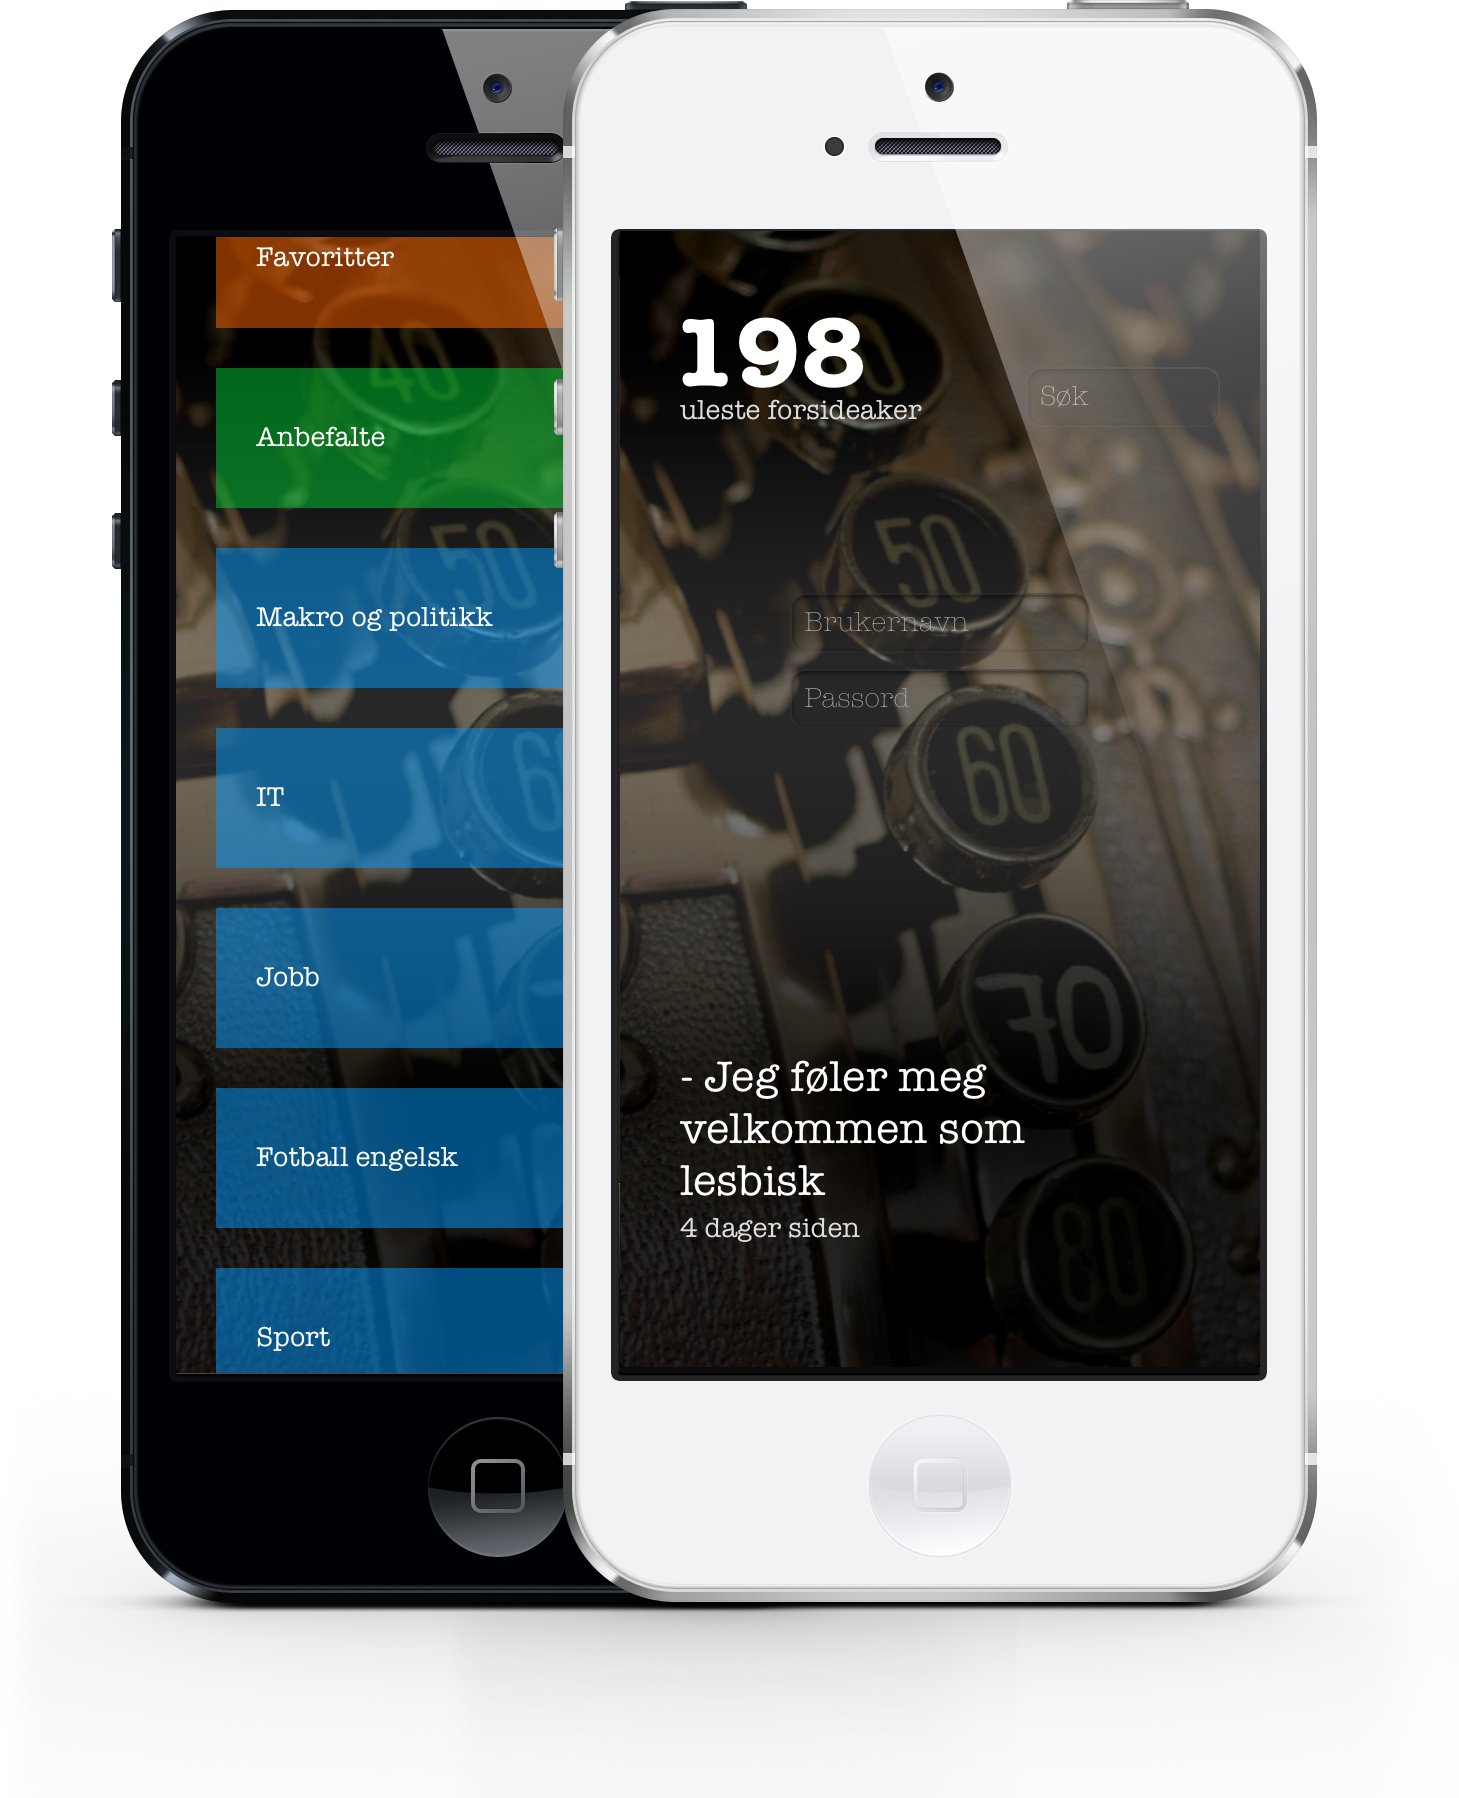
\includegraphics[width=120mm]{GFX/clientApp/categoryAndFrontPage.png}
\caption{Screenshots from the client application showing the start page and the category selection screen.}
\label{screenshots_nyhetene_start_and_category}
\end{figure}

The categories in the category selection screen are categories that are defined by the back-end by analyzing the article's content, as well as the categories set in the RSS feeds provided by the content publishers. The user can also access any stored articles from this menu. By clicking a category in the category selection screen the RSS view will be presented showing the articles from the category clicked. The RSS view is shown in figure \ref{screenshots_nyhetene_rss_and_share}. 

\begin{figure}[!htbp]
\centering
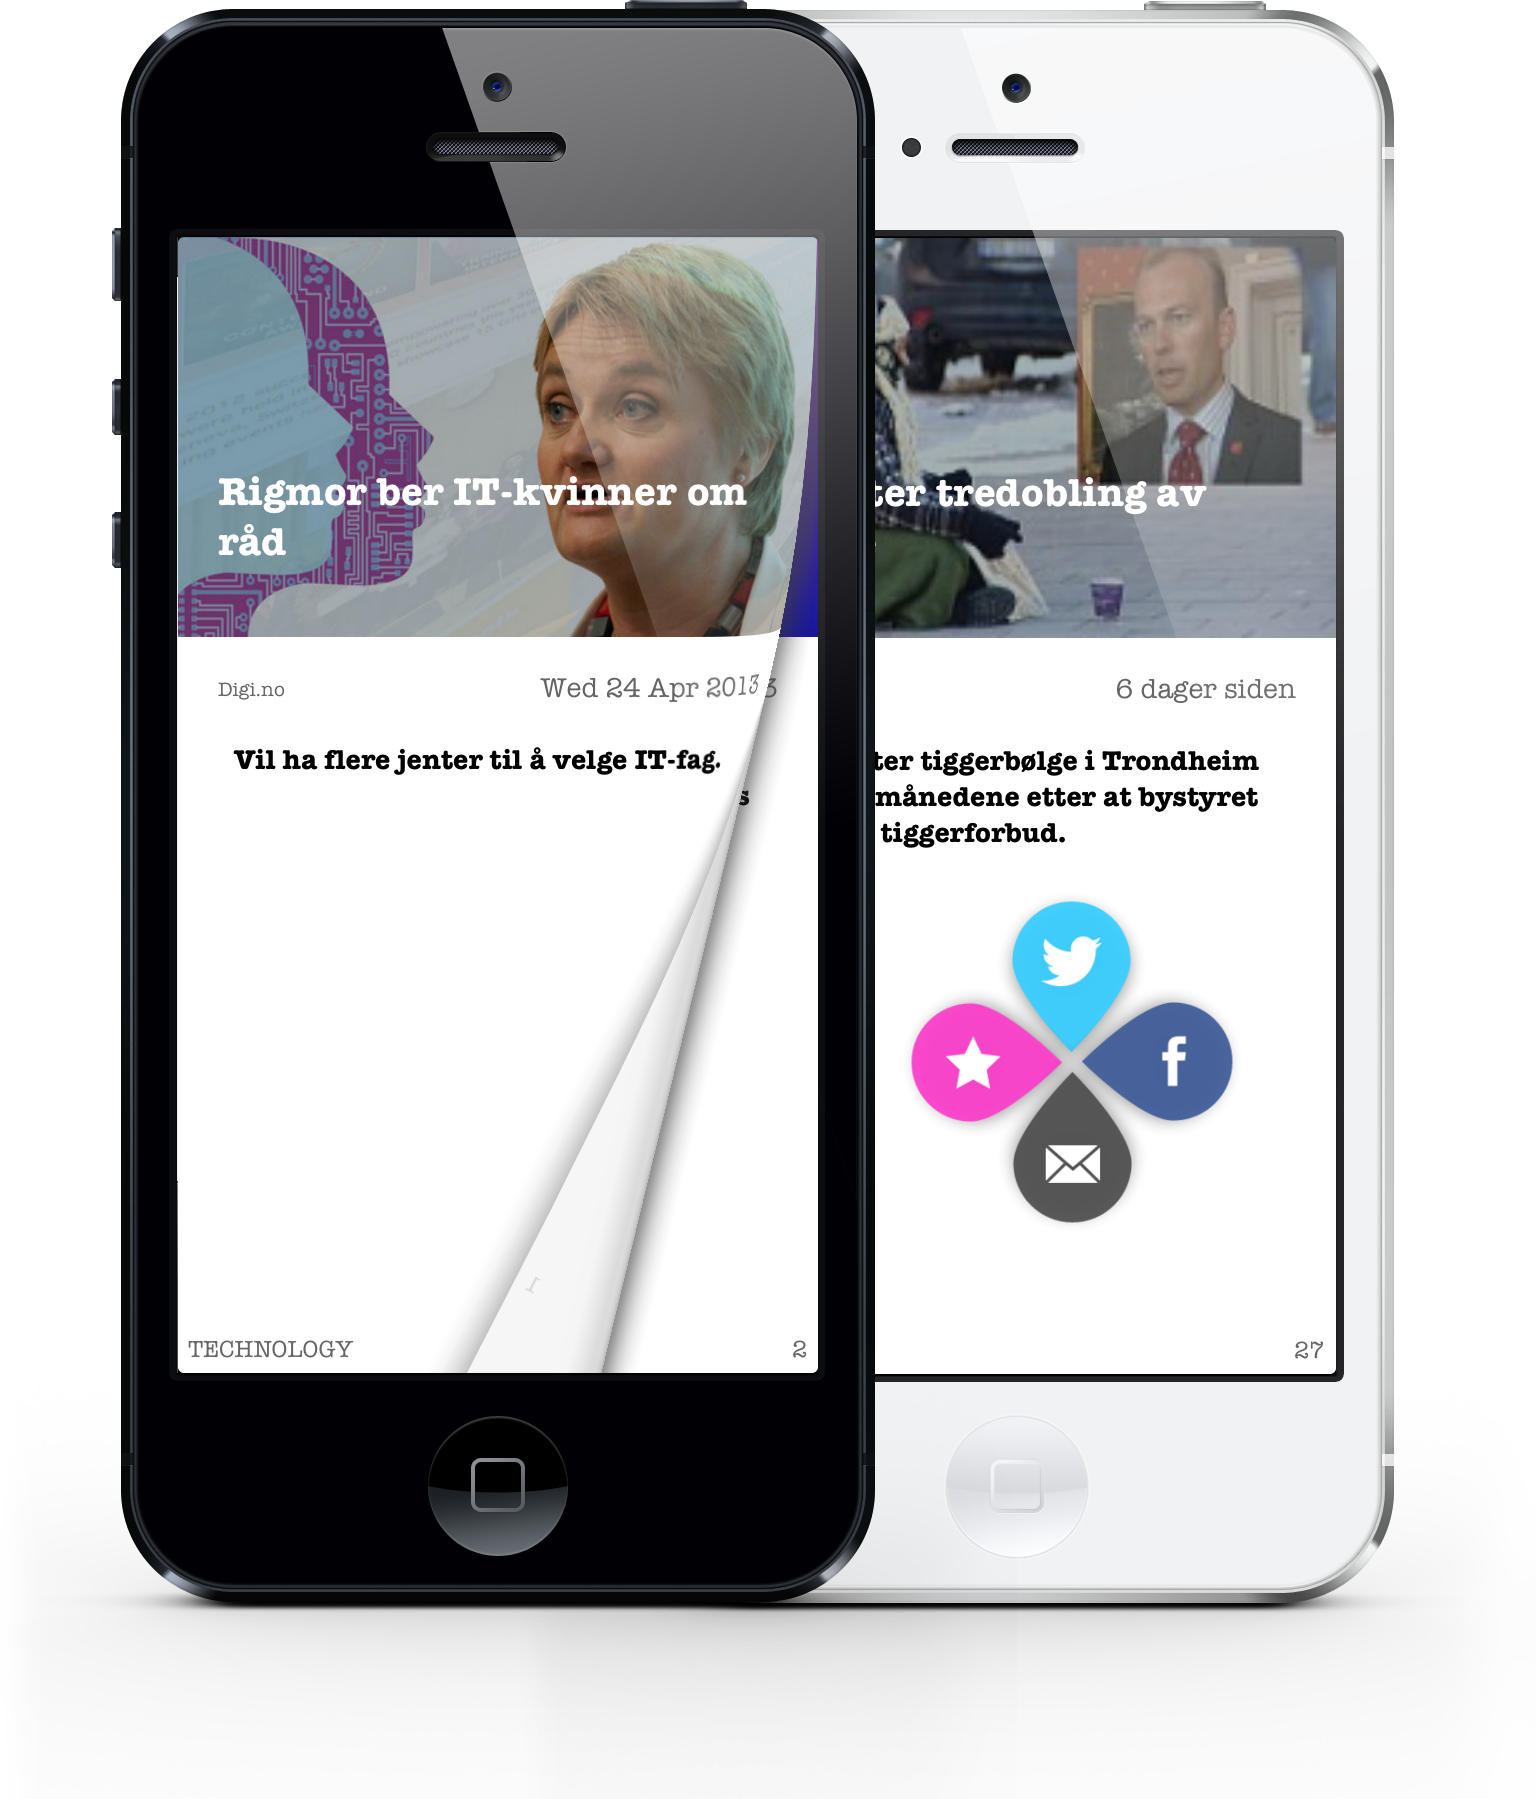
\includegraphics[width=120mm]{GFX/clientApp/rssViewAndShare.png}
\caption{Screenshots from the client application showing the RSS view and the RSS view after triggering the share/save menu.}
\label{screenshots_nyhetene_rss_and_share}
\end{figure}

At the top of the RSS view the title of the article is shown on top of the article's image, if any. The view also shows the publisher, when it was published, which categories the article resides to, the page number the article has of all the articles retrieved in this category and the lead text. To navigate back and forth between the different articles, a horizontal swipe is used. A double tap anywhere on the screen will trigger an update of the news in this category and bring the user to the foremost article. The share/save menu, as shown in the rear image in figure \ref{screenshots_nyhetene_rss_and_share}, is triggered by holding down one finger anywhere on the screen for a short amount of time. From this menu the user can share the article via Facebook, Twitter or mail, as well as storing the article for later reading, by tapping the star icon. By swiping up in this screen the user will be sent back to either the category selection screen or the start screen, depending on which of the two screens triggered the presentation of the RSS view. By swiping down on the RSS view, the full article view is presented to the user. The full article view is shown in the foremost image in figure \ref{screenshots_nyhetene_full_article_and_map}


\begin{figure}[!htbp]
\centering
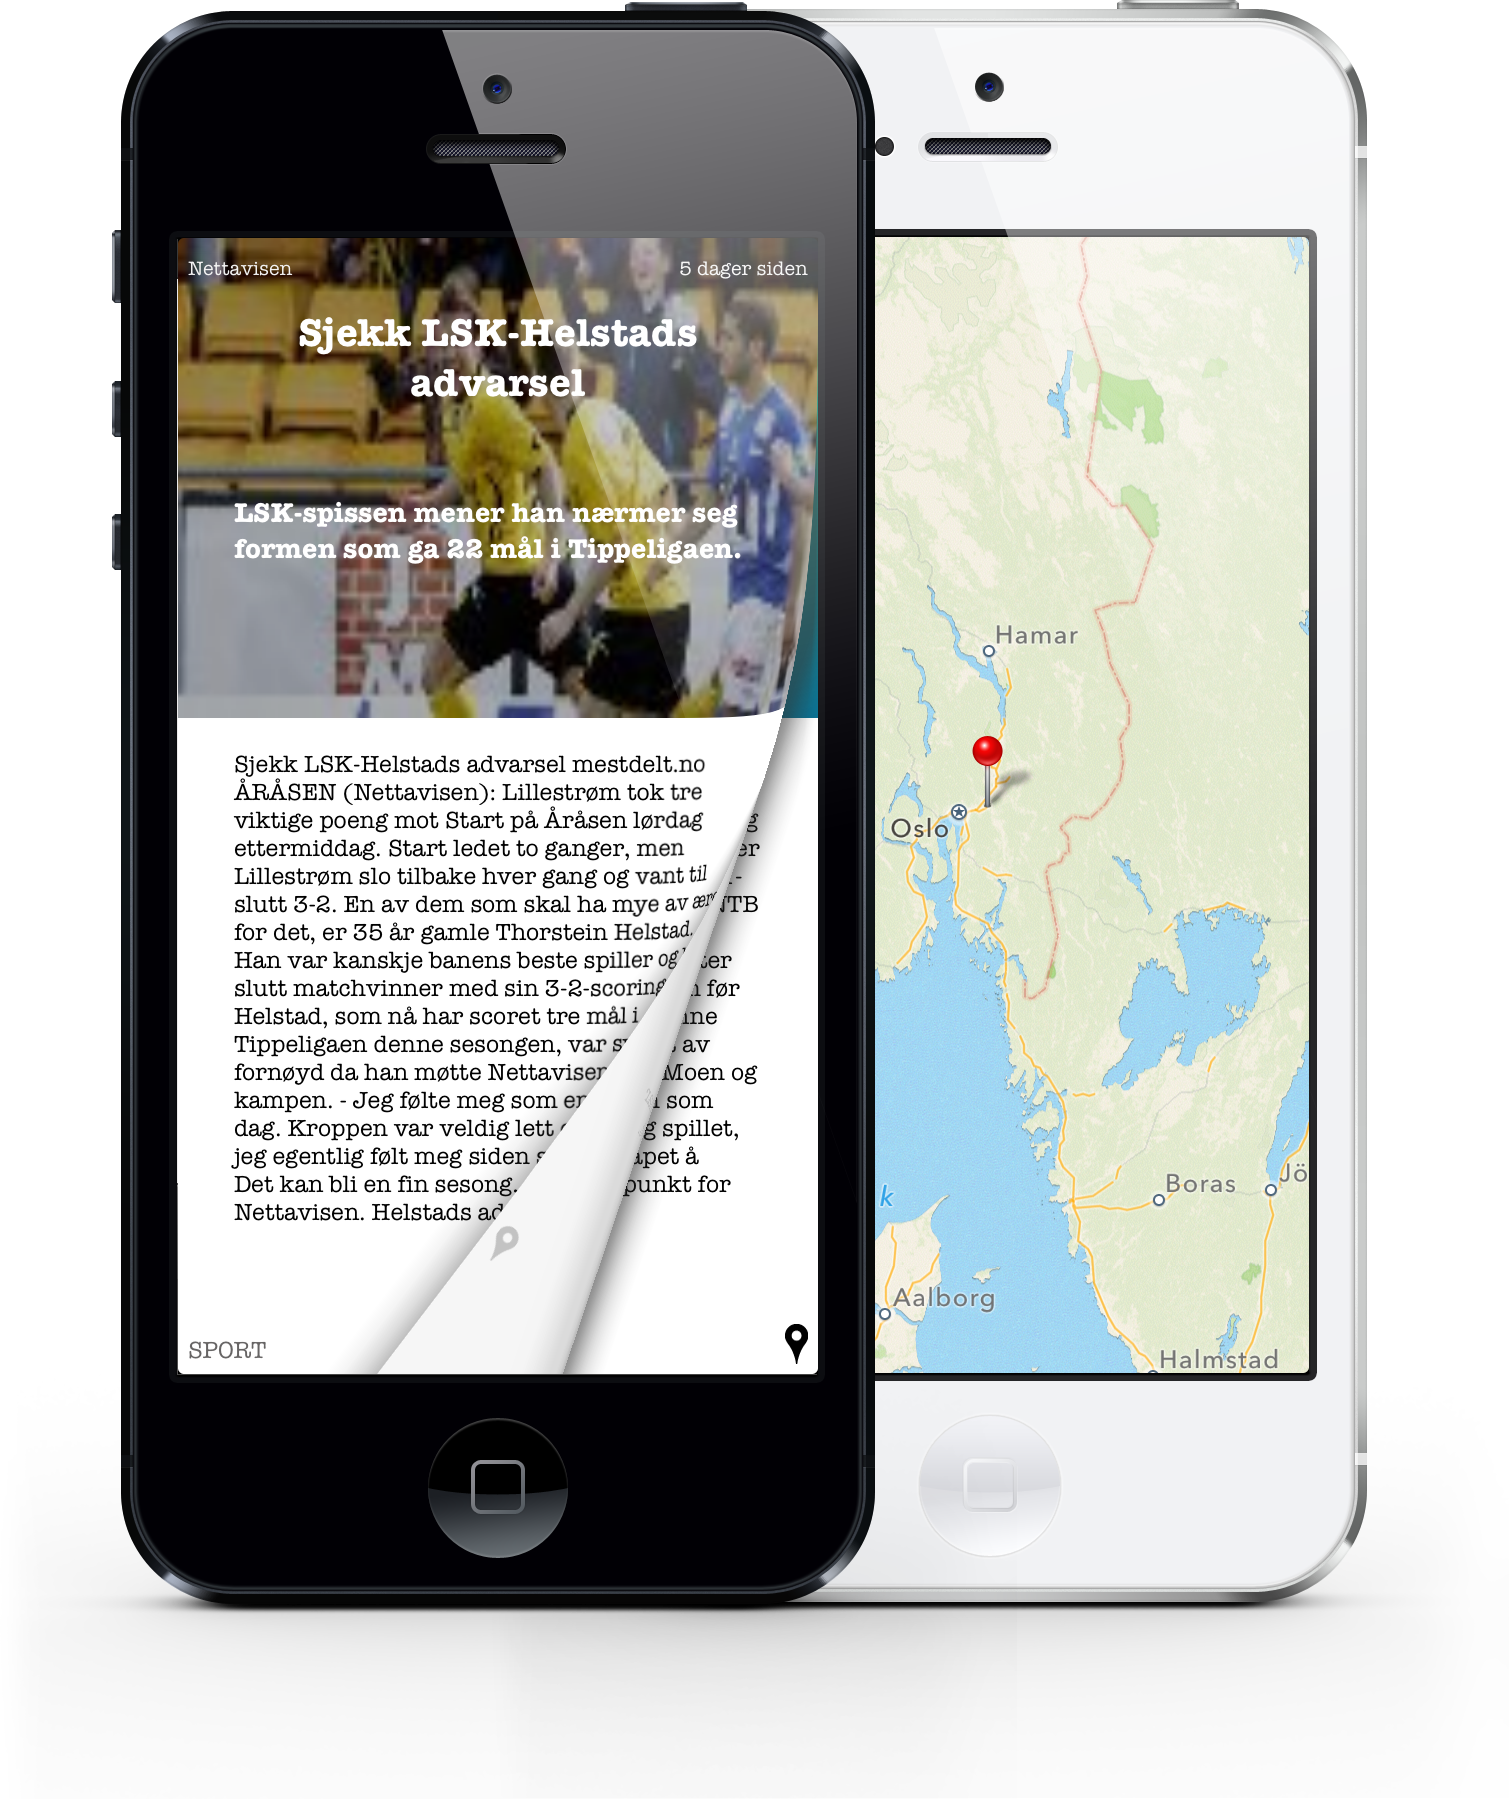
\includegraphics[width=120mm]{GFX/clientApp/swipeForSimilarAndMap.png}
\caption{Screenshots from the client application showing the full article view and the map view.}
\label{screenshots_nyhetene_full_article_and_map}
\end{figure}


The full article view are quite similar to the RSS view, but in addition to all the information found in the RSS view, the full article view has access to the full article text, related articles and the possibility to show where the article resided on a map. The start of the full article text is shown in the lower part of the screen, and if the user wants to continue reading the the article text, a press and hold with one finger anywhere on the screen will bring up a new view showing only the article text in a full screen format. Here the user can read the whole story without minding any other information besides the article text. To close the article text view the user holds down one finger for a short amount of time again. If the article has any locations connected with it, a map pin is shown in the bottom right corner of the screen. By tapping this map pin or by double tapping the screen, a full screen map view (rear image in figure \ref{screenshots_nyhetene_full_article_and_map}) is presented showing on a map, all the locations that are connected with this article. To close the map view, the user simply double taps it again. The back-end system also delivers related articles to any article retrieved, if there exist any. These can be viewed by performing a horizontal swipe, similar to the RSS view. The related articles are shown in the same way as the full article view.

As mentioned earlier, the settings view are presented when performing a swipe up gesture in the start screen. The settings view shows how the user profile is stored in the back-end system, with regard to which criteria that are weighted most when retrieving news. These criteria are freshness and location, for instance. These values are set by the back-end system based on the user activity, and the user has the ability to override these settings and storing them, as well as wiping the user profile clean and start the learning from scratch. The user can also override the GPS location if the user wants news from a different place than where the device is currently residing.


\subsection{Technology}
The SMNRS, as shown in figure \ref{tech_news_app_architectural_view}, is quite complex and consists of several advanced technologies and APIs.

\subsubsection{Back end}
The back end starts by subscribing to different RSS feeds, consisting of different publishers and categories, provided by various news content providers. The preprocessing part consists of six steps:

\begin{enumerate}
	\item Extract RSS entries
	\begin{itemize}
		\item The RSS entries are extracted using an RSS parsing library for Java, called ROME.
	\end{itemize}

	\item Download HTML contents
	\begin{itemize}
		\item The news pages are scraped using a library called Apache Tika.
	\end{itemize}
	
	\item Extract body text
	\begin{itemize}
		\item Extraction of the body text are done using the same library as for downloading the HTML contents, Apache Tika.
	\end{itemize}
	
	\item Named Entity Recognition
	\begin{itemize}
		\item For the NER, a library called Apache OpenNLP is used, and the model used is especially trained for the Norwegian language.
	\end{itemize}
	
	\item Geo Code tagging
	\begin{itemize}
		\item Geo Code tagging is realized through the Google Location API.
	\end{itemize}
	
	\item Index document
	\begin{itemize}
		\item The documents are indexed in an Apache Solr solution, which supports queries that combine geographical and content-related elements.
	\end{itemize}
	
\end{enumerate}

Further these news article documents are stored in a search engine/document store service, using Apache Solr\footnote{Apache Solr stems from the Apache Lucene project and provides an open source enterprise search platform. More information at \url{http://lucene.apache.org/solr/}.}.

To be able to get recommended news based on user activity and preferences, user profiles and user event logs are stored in a MongoDB\footnote{MongoDB is a type of database for storing structured data. More information at \url{http://www.mongodb.org/}.}. An Apache Hadoop\footnote{Apache Hadoop is a framework for distributed processing of large data sets. More information at \url{http://hadoop.apache.org/}.} batch job is running to constantly process the user events and updating the user profiles in the MongoDB.

A middleware layer is put on top of the Solr and MongoDB systems using a REST API\footnote{A REST API is way of providing an interface to underlying technologies to make it easier to retrieve and store information without worrying about how the underlying technologies communicate.} to make querying news, storing event logs and updating user profiles an easier and more universal task.

\subsubsection{Client}
To retrieve the recommended news, the client queries the REST API for news, providing the back end with an unique user id and geolocation to get the news that best fits the user and the user's location, represented as JSON objects. If the user clicks a category, the category string is added to the query and if the users opens an article in the full article view, the client application queries the REST API for related news providing a news article id, in addition to the user id and geolocation.

The client also tracks the user's activities, like if the user opened the full article view of an article, this counts as a positive event for this category or topic and will affect the user's profile. Which again will have an impact on the news delivered to this user. These events are pushed and stored in the MongoDB via the REST API every time the client makes a news query, and further processed by the Hadoop batch job, which will update the user profile according to the events pushed.

\begin{figure}[!htbp]
\centering
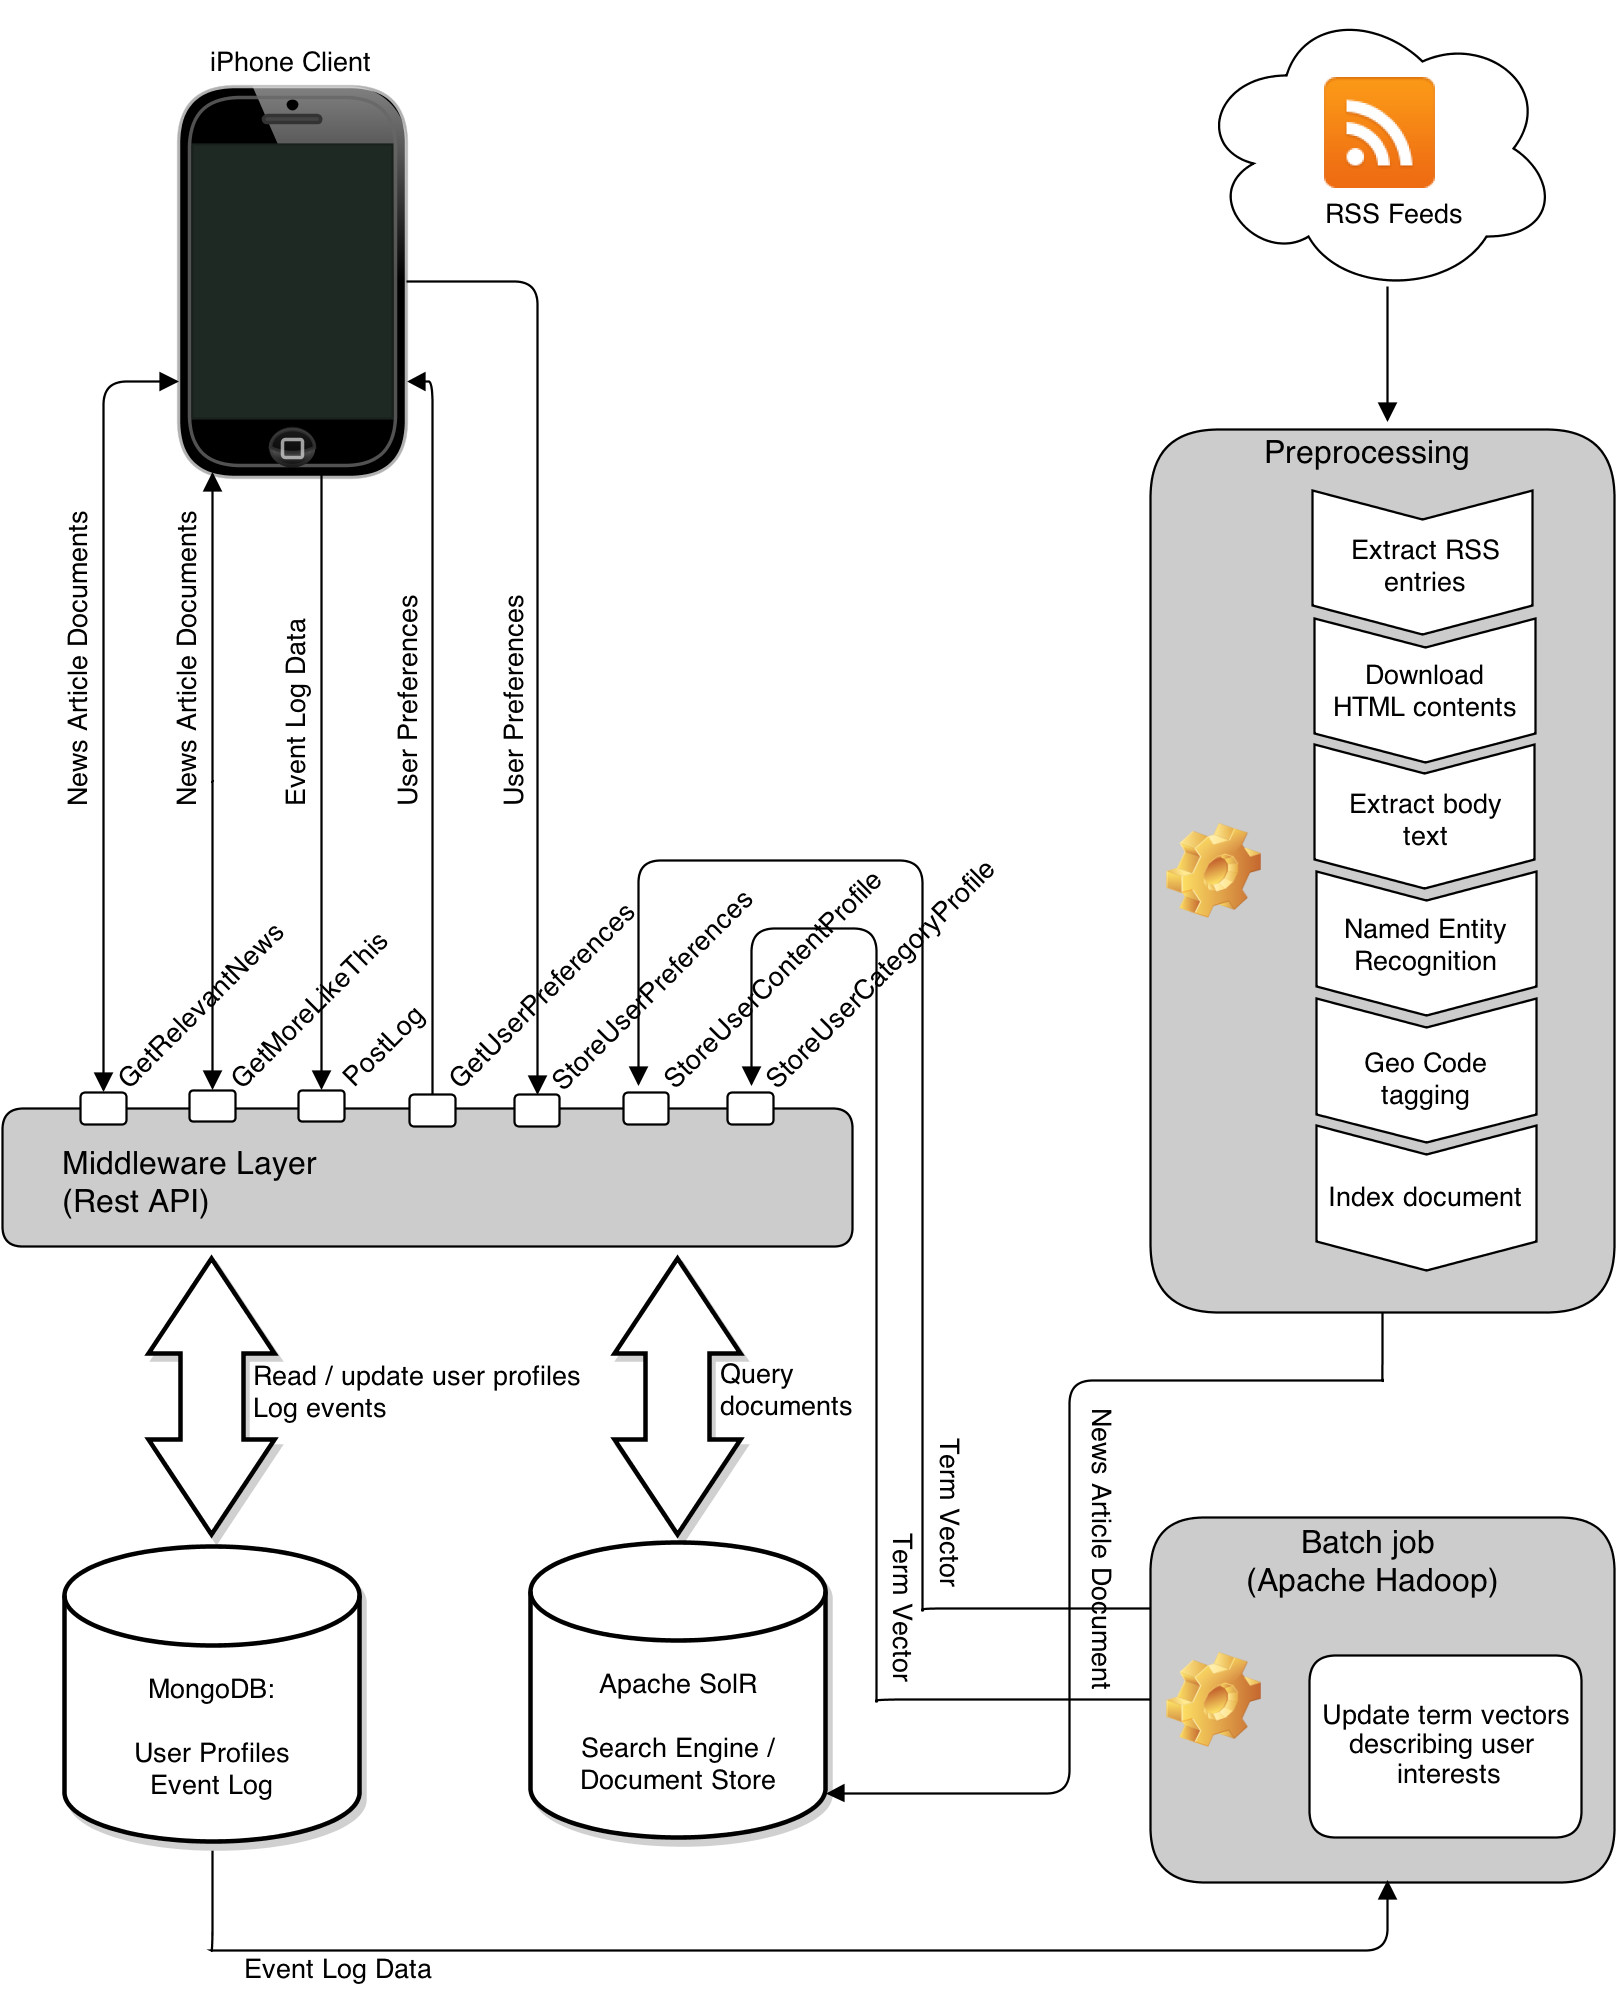
\includegraphics[width=150mm]{GFX/tech/newsAppArchitecture.png}
\caption{Conceptual drawing showing the architectural view of the whole Smartmedia Mobile News Recommender System.}
\label{tech_news_app_architectural_view}
\end{figure}